%!TEX root = main.tex

\section{Experimentation and Evaluation Plan}
\label{sec:experiment}

% \begin{itemize}
%     \item We need to describe in detail all the experiments and testbeds we will use/develop.
%     \item this is emphasized int he solitication
%     \item describe how we will recruit subjects
%     \item emphasize the real world experimentation plan
% \end{itemize}

% \textit{This section should describe how the research concepts proposed will be demonstrated and validated. It should present metrics for success. It should identify critical experiments, and describe how the research will be demonstrated, including through simulation, prototyping, and integration with real (including sub-scale) cyber-physical systems. For Medium and Frontier projects, the validation plan must include experimentation on an actual cyber-physical system.}

%\lu{Lu describes the full scale driving simulator}


Each of the proposed research thrusts in Sections~\ref{sec:behaviour},\ref{sec:reachability}, and \ref{sec:feedback}, we will conduct extensive experimentation using high fidelity automobile simulators like PreScan and AirSim, a full scale diving simulator, smaller scale autonomous vehicle test-beds, and a full scale car fitted with sensors for monitoring human driving behavior and emotions. We next describe in detail, the different cyber-physical systems tesbeds, and a cross cutting experimentation plan for the three research thrusts. 


\subsection{Scenario-based behavior and trust modeling}
\label{subsec:trust-modeling}
\begin{figure}
    \centering
    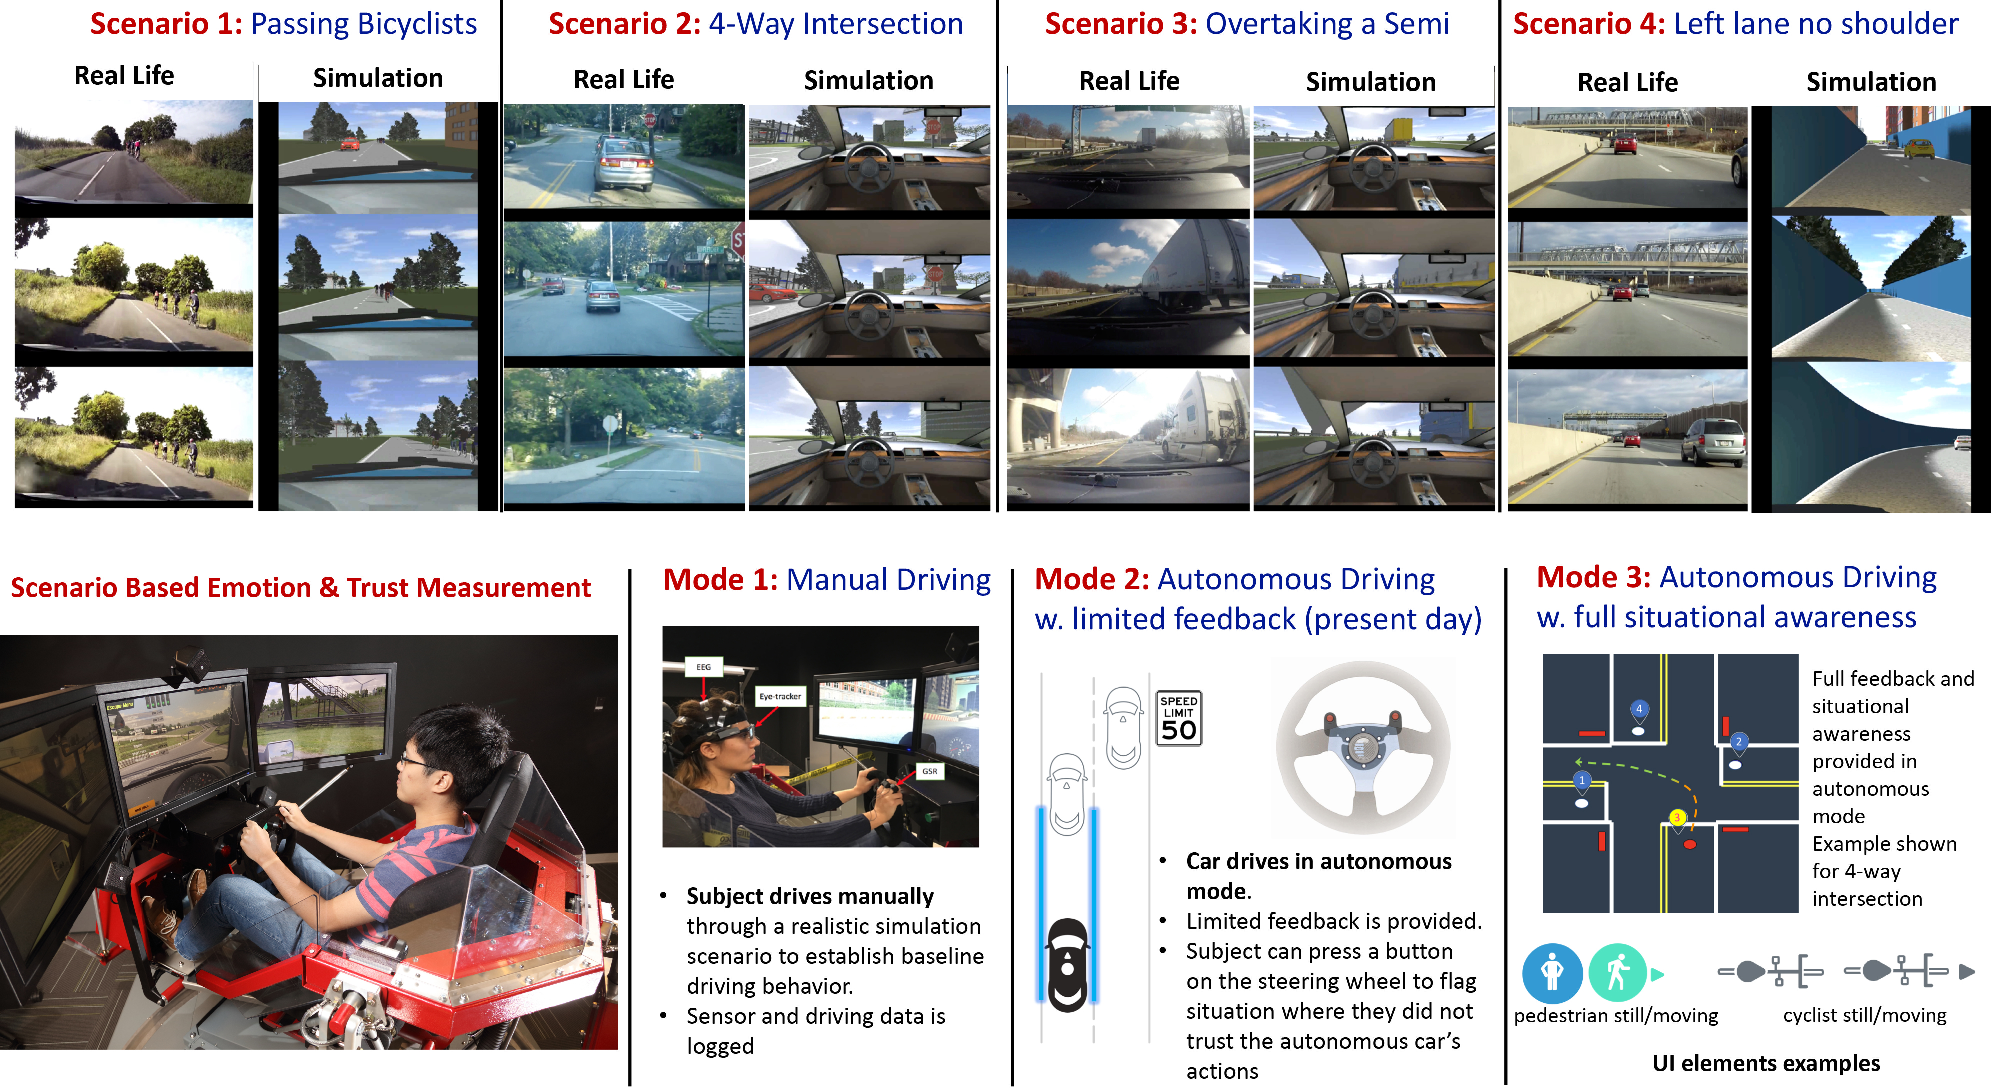
\includegraphics[width=\columnwidth]{figures/scenarios.pdf}
    \caption{Overview of the Scenario Based Emotion and Trust Measurement - We recreate real world traffic situations in simulation using Pre-Scan. During experimentation, we invite human drivers to first manually drive through each scenario (mode 1), followed by an autonomous driving mode where limited feedback and car intentions are provided to the driver, and finally in mode 3, the users experience fully autonomous driving with full feedback and situational awareness provided. We then survey the participants about what feedback enables their trust, which UI elements do they prefer, which mode made them emotionally satisfied.  }
    \label{fig:scenario}
\end{figure}

Behind the wheels of a self-driving car, everyone of a sudden becomes a backseat driver. For thrust 1 on monitoring driver behavior and emotions (Section~\ref{sec:behaviour}, we want to observe and record driver activity in a controlled environment. 
For thrust 3 on feedback design (Section~\ref{sec:feedback}), we want to measure how passengers react to varying degrees of feedback and explanations provided to them by the UI. We setup different traffic scenarios in our full scale driving simulator, to run experiments to gather the data required to build models for human behavior, and test the effectiveness of different kinds of feedback. 
We can simulate multiple scenarios – a four way stop sign, safely passing bicyclists on a narrow road, overtaking a large semi on a freeway, driving too close to a barrier in the absence of a shoulder on the left lane, etc. 

\subsubsection{Participants}
We are proposing to conduct user studies and driving experiments for Thrusts 1, and 3.
The design of a subject study protocol is being undertaken at the time of the witting of the proposal. We are closely working with the Institutional Review Board for Social and Behavioral Sciences at the University of Virginia. The data management plan describes in detail how user data will be recorded, used, distributed, and maintained. A total of at least 100 participants from the University of Virginia will be recruited for participation in this study over 3 years. We we take measures to ensure sufficient diversity within the participation pool. Subjects will be awarded in exchange for participation in accordance with the University of Virginia’s Institutional Review Board practices, and we have requested a budget for the same.


\subsubsection{Setup}
Figure~\ref{fig:scenario} shows the setup of an academic-scale testbed that co-PI Feng's group has partially built and will complete during the proposed effort. The hardware platform is based on the Force Dynamics 401CR driving simulator. This four-axis motion platform can pitch, roll, yaw, and heave, to simulate the experience of being in a vehicle. Thus, we expect to collect data about realistic human response during the driving. The human is interfaced to the hardware platform through PreScan, which is a software tool designed as a development environment for Advanced Driver Assistance Systems (ADAS) and Intelligent Vehicle (IV) systems. PreScan supports virtual sensor technologies such as radar, laser, camera, ultrasonic, GPS and C2C/C2I communications. 
Sensors will be used for both high-level inference of human's intent and preferences and low-level monitoring of human behavioral, mental and physiological states. These sensors include EEG for neural signals, EKG for heart activity, EMG for muscle activity, a camera for head tracking, eye tracking suite and cloud-based speech recognizer.

\subsubsection{Design and procedure}

As shown in Fig.~\ref{fig:scenario}, we have re-created 4 real world driving situations in Pre-Scan - passing bicyclists on a narrow back road, a 4 way intersection, overtaking a semi truck at freeway speeds, and driving on a  freeway in the left lane in the absence of a left shoulder. 
For each of these scenarios, we will conduct the following user experiment:
\begin{enumerate}[itemsep=0pt,parsep=0pt,topsep=4pt,leftmargin=0.4in]
    \item Mode 1 - Manual driving: In this mode, we ask the subject to drive through a given scenario. Each scenario's simulation is a few minutes. While they drive through the scenario, we monitor the person's behavior and emotional cues as well as log their driving behavior. This driving behavior ( steering, brake, acceleration) can be considered as their baseline profile. We also track their gaze, to asses what the driver is paying attention to as they drive. As an example, we will ask the subject to drive through the four way stop sign scenario, where they have to self-asses their right of way as they approach a stop sign. We can then intentionally program one of the agents in the simulation to drive3 out of the order for the right of way and see how the driver adapts. 
    \item Mode 2 - Autonomous driving with limited feedback: Next, we ask the same subject to this time, sit back and relax, as the car drives by itself in the simulator. Everything in the scenario is identical to last time, except that the driving is fully autonomous. We present the driver with a visualization of a virtual dashboard which depicts what the car sees, very similar to what most of the dashboards for semi-autonomous vehicles depict today.  Once again, we monitor the drivers behavioral and emotional cues to interpret their trust in the system. We also give them the option to press a button on the steering wheel, every time they think the car did something that they did not anticipate, or if they mistrusted the car's autonomous driving actions. ``flagging'' these events in a scenario provides us with a basis for designing UI feedback. Continuing with our previous example, a visualization of the four way stop sigh is shown the viewer as feedback, but no indication is given as to if the autonomous car has figured out its right of way, or what is its intended trajectory.
    \item Mode 3 - Autonomous driving with full feedback: Lastly, we have the autonomous car drive through the same scenario one more time, but this time we provide full situational awareness of the scene to the user along with cues about the car's intended actions. In the stop sign example, we project the car's understanding of its right of way, and how that dynamically updates as other vehicles drive through the intersection. We project the cars intended trajectory so the user know that the car will make a left turn and will yield to incoming traffic. More generally, for the parts of the simulation which were flagged by the user, we run the Deep Explanations engine to provide natural language explanations for the car's actions. 
    
\end{enumerate}

Following the experiment, we survey the subjects to understand and gather data on which explanations help increase the trust of the subject, which UI elements work, and to what extent.
Each participant will also be given a questionnaire, adapted from~\cite{merritt2013trust}, to learn about their levels of trust in the autonomous car. 
We will use scales which empirically define the feeling of trust in the autonomous system from~\cite{jian2000foundations} which has been used in many studies about trust~\cite{hoff2015trust}.

\subsubsection{Expected results} 
Upon the completion of data collection, the data will be subjected to a factor analysis to reveal the underlying factor structure of the experimental scale. 
The goal of factor analysis is to condense a larger set of variables to a smaller set of factors, which account for a sizeable proportion of variability within the items. Thus, it is desirable to have a few factors that account for a large portion of the variance. 
A one-way analysis of variance (ANOVA) will also be conducted to examine differences in trust amongst the different driving modes. 
It is anticipated that there will be differences in trust depending on the subject's preferences, driving style, and the autonomous car's behavior. 
More specifically, we anticipate that trust will attenuate with higher levels of feedback. We will create a library of UI elements, a library of simulation scenarios, with detailed statistics about which elements worked and what was the subject's assesment.

In addition, the simulated scenario based experimentation will enable:
\begin{enumerate}[itemsep=0pt,parsep=0pt,topsep=4pt,leftmargin=0.4in]
    \item Creating a library of emotional profiles, and models, of drivers.
    \item Identifying the mapping between the emotional state and the control action of the autonomous car, and vice-versa.
    \item Collect valuable data for training the Deep Explanations networks for natural language feedback.
    \item By deploying the same subject in a real car and monitoring their preferences and driving behavior, we will also validate the realism of the simulation study. 
\end{enumerate}

Although, the simulation setup has a distinct advantage, i.e. repeatability of the same scenario, one of the goals of the proposed work is to develop the proposed models for emotion and driving behavior using data from a real deployment in a car (described later in this section). 







% \begin{figure}[t]
% \centering
% \includegraphics[width=.9\textwidth]{figures/testbed}
% \caption{Our partially built testbed of human-autonomous vehicle interactions. The human is monitored by a number of sensors, and interacts with the driving simulator through the PreScan software interface.)} 
% \label{fig:testbed}
% \end{figure}

 %These are systems with sensors that monitor the vehicle's surroundings and that use the acquired information to take action. Such actions may range from warning the driver of a potentially dangerous situation to actively evading hazards by means of automatic braking or automatic steering. 
% The ``human monitoring and sensing'' block in Figure~\ref{fig:testbed} encloses the sensors that will be used for both high-level inference of human's intent and preferences and low-level monitoring of human behavioral, mental and physiological states. These sensors include EEG for neural signals, EKG for heart activity, EMG for muscle activity, a camera for head tracking, eye tracking suite and cloud-based speech recognizer.

\subsection{Test-beds for reachability and control synthesis experiments}

%\nicola{Nicola describes the experiment setup for reachability analysis experimentation}

\begin{wrapfigure}{R}{0.35\linewidth}
\vspace{-5pt}
\centering
\includegraphics[width = \linewidth ]{figures/jackal_2.jpg} 
\caption{one of the autonomous ground vehicles available in PI Bezzo's lab to validate the proposed research.}
\vspace{-5pt}
\label{fig:jackal}\end{wrapfigure}

\subsubsection{Autonomous ground vehicles}
The proposed research, in particular Thrust 2 about safety assessment via reachability analysis and and reconfiguration via safe reinforcement learning will be validated using our testbed of autonomous ground vehicle available in PI Bezzo's robotics laboratory. Figure~\ref{fig:jackal} shows one of the autonomous ground vehicle equipped with the same sensors available in real autonomous cars which include velodyne lidar, stero cameras, imus, wheel encoders, differential GPS, and onboard i7 cpu. The vehicle's equations of motion and dynamics are similar to real autonomous vehicles with reduced speed. This platform and especially the sensor testbed will be used offline to create a library of primitives for the reachability analaysis and then used at runtime in different scenarios to predict and validate the safety assessment presented in Thrust 2. We also plan to use virtual reality goggles (also available in the PI's lab) to simulate the presence of a human on board the vehicle. 

\subsubsection{1/10 scale autonomous vehicle testbed}

PI Behl has developed a 1/10 scale autonomous racing car platform called F1/10~\citeN{f1tenth}. The cars are a realistic representaiton of a full scale car, with similar dynamics, just different parameters. It carries a suite of sensors similar to that carrier by current full scale prototypes of autonomous vehicles, including a LIDAR, a stereo camera, depth camera, an IMU, and a high performance GPU board running the Robot Operating System (ROS).
PI Behl has built a fleet of F1/10 cars and has access to an indoor track facility for testing the control synthesis algorithms in a safe environment but at high and realistic traffic speeds. The PI also has access to a 1/10 scale car which has been modified in that it can be driven in first person view (FPV) using steering wheels and pedals, while wearing a headset which relays the onboard camera view to the human driver, thereby allowing us to conduct both UI and driving style behavior experiments at 1/10 the scale.



%\madhur{Madhur describes F1/10 - could be used for reachibility + control synthesis}